\section{PDE3: 2D Shallow Water Equations for the Tohoku 2011 Tsunami}
\label{sec:SWE-Tohoku}

\renewcommand{\thefigure}{E.\arabic{figure}}  % Number figures as A.1, A.2, ...
\renewcommand{\thetable}{E.\arabic{table}}  % Number tables as A.1, A.2, ...


\subsection*{Overview}
We evaluate the feasibility of near-real-time large-scale tsunami inversion and forecasting using SC-NOs, governed by the hyperbolic Shallow Water equations, based on the 2011 Tohoku event. Variability arises from earthquake-induced seafloor deformation computed using the Okada model \citep{grilli2013numerical} with different geometries and epicenter locations. We use noise-contaminated synthetic water-level observations at sea-buoy locations from the first 30 minutes as observations for the inverse source identification, followed by forward forecasting. The inversion first estimates an initial guess of the seafloor deformation field, restricts it to the Okada representation, and then optimizes the Okada model parameters via the pretrained neural operators (Methods). All neural operators (FNO and SC-FNO) are pretrained on high-resolution simulations from a observationally-validated finite-volume solver (Supplementary Figure~\ref{fig:tohoku_validation}), coarsened to the NO grid resolutions. They receive deformation fields $\Delta z_b(\mathbf{x})$ and an initial water stage ($t_u = 1$) as inputs and predict the remaining $t_G = 50$ time steps. We calculate the sensitivity (Jacobian) of the final water stage with respect to bed topography using adjoint-sensitivity analysis.


\subsection*{Problem setup}
We solve the shallow water equations (SWE) with Manning friction over a two-dimensional ocean domain \( \mathcal{X} = [0, L] \times [0, L] \) and time \( t \in [0, T] \). This formulation captures wave propagation, coastal inundation, and wet-dry dynamics. Given spatial coordinates \(\textbf{x} = (x, y) \in \mathcal{X} \), the governing SWE system is:



\begin{equation}
\frac{\partial}{\partial t}
\begin{pmatrix}
h \\[3pt]
m_x \\[3pt]
m_y
\end{pmatrix}
+ \nabla \cdot
\begin{pmatrix}
h \mathbf{u} \\[5pt]
h u \mathbf{u} + \tfrac{1}{2}\,g\,h^2 \,\mathbf{I}_x \\[3pt]
h v \mathbf{u} + \tfrac{1}{2}\,g\,h^2 \,\mathbf{I}_y
\end{pmatrix}
=
\begin{pmatrix}
0 \\[4pt]
-\,g\,h\,\frac{\partial z_b}{\partial x} \;-\; \bigl(\text{friction}_x\bigr) \\[6pt]
-\,g\,h\,\frac{\partial z_b}{\partial y} \;-\; \bigl(\text{friction}_y\bigr)
\end{pmatrix}.
\end{equation}

Here, \( h \) is the water depth, \( \mathbf{m} = (m_x, m_y) = (h u, h v) \) is the depth-integrated momentum, \( \mathbf{u} = (u, v) \) is the velocity, and \( z_b(x, y) \) represents the bed elevation. The source terms include the bed slope and Manning friction:

\begin{equation}
\text{friction}_x = g n^2 \|\mathbf{u}\| \frac{h u}{h^{7/3}}, 
\quad
\text{friction}_y = g n^2 \|\mathbf{u}\| \frac{h v}{h^{7/3}}.
\end{equation}
To represent wet-dry dynamics, dry regions are modeled by setting \( h = 0 \) when the water depth falls below a threshold. no reflection boundary conditions are imposed in both \( x \) and \( y \) directions to simulate an open ocean. 

\subsection*{Modeling Seafloor Deformation Using the Okada Dislocation Model}
The Tohoku 2011 tsunami was triggered by an Mw 9.0 earthquake along the Japan Trench on March 11, 2011. To simulate this event, we investigate a 1000 km × 1000 km region as illustrated in Figure \ref{fig:bed_elevation}, using real bathymetry data to define the pre-earthquake seabed topography \( z_{b0}(\textbf{x}) \). This dataset, obtained from ETOPO 2022 at 30 Arc-Second resolution, provides an accurate baseline representation of the ocean floor before the earthquake.

% Begin the figure environment
\begin{figure}[htbp]
    \centering
    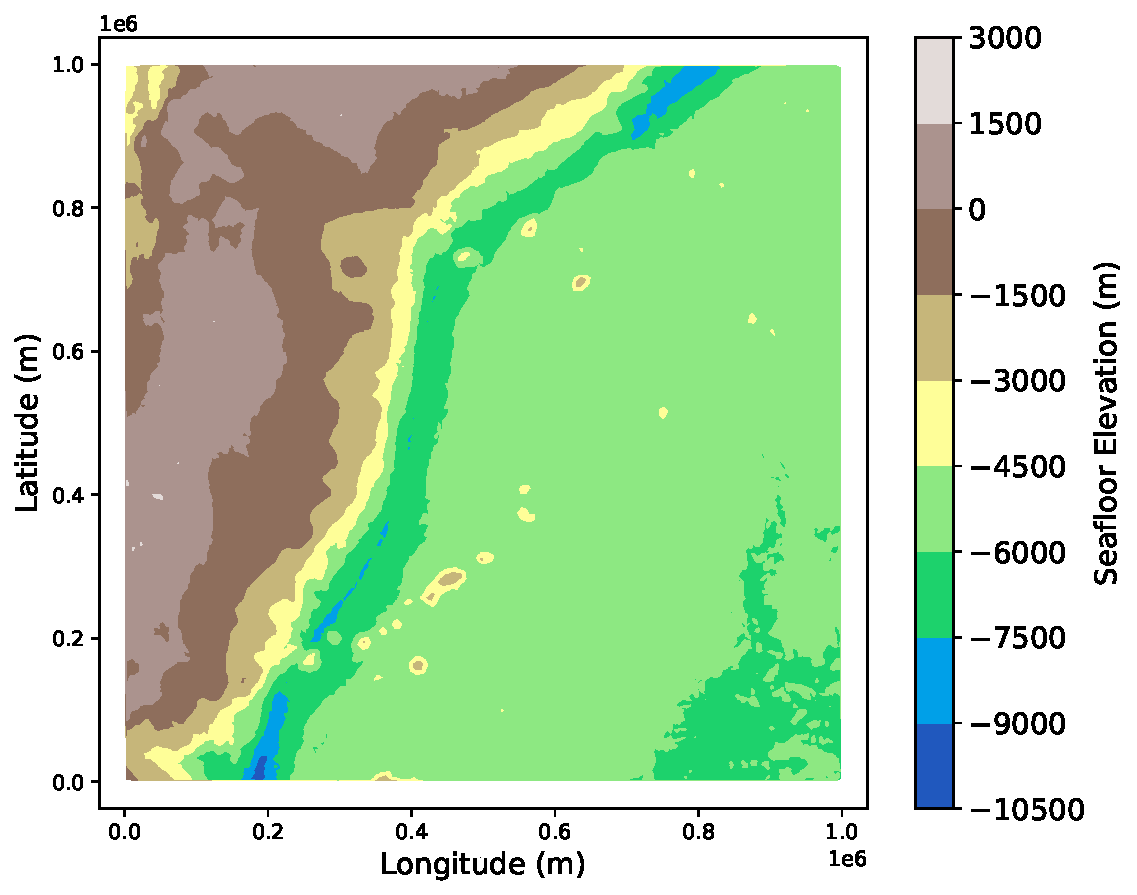
\includegraphics[width=0.65\textwidth]{Figuers/bed_elevation_raw.pdf} % Adjust width as needed
    \centering
    \caption{\scriptsize Bathymetry and Topography of the Computational Domain for the 2011 Tohoku Tsunami Simulations}
    \label{fig:bed_elevation}
\end{figure}

% Reference the figure in your text
As shown in Figure~\ref{fig:bed_elevation}, Bathymetry of the Computational Domain for the 2011 Tohoku Tsunami simulations. Before the earthquake, the water surface is assumed to be at rest, with an undisturbed sea level and no initial flow:

\begin{equation}
h(\textbf{x}, 0) = 0, \quad u(\textbf{x}, 0) = 0, \quad v(\textbf{x}, 0) = 0.
\label{eq:swe-initial-prequake}
\end{equation}
To model the seafloor deformation caused by the earthquake, we use the Okada displacement model \citep{okada1992internal}, which provides an analytical solution for surface deformation due to fault slip in an elastic half-space. This model computes the coseismic displacement \( \Delta z_b(\textbf{x}) \) based on key fault parameters that define the fault geometry and slip characteristics. The \textbf{depth} represents how deep the fault's top edge is below the surface, while the \textbf{length} and \textbf{width} describe the along-strike and down-dip dimensions of the fault plane. The \textbf{slip} quantifies the magnitude of displacement along the fault, whereas the \textbf{strike} specifies the fault's orientation relative to north, measured in degrees. The \textbf{dip} represents the inclination angle of the fault plane relative to a horizontal surface, while the \textbf{rake} defines the direction of slip along the fault plane. Together, these parameters determine the vertical displacement field, shaping the seafloor uplift or subsidence that drives tsunami generation. The earthquake's epicenter location is defined by its \textbf{\( x \)-coordinate} and \textbf{\( y \)-coordinate}, determining the origin of the deformation. Given these parameters, the Okada model computes the vertical displacement field \( \Delta z_b(x) \), representing the seafloor uplift or subsidence that alters the initial seabed topography. This deformation is incorporated into the model as:

\begin{equation}
z_b(\textbf{x}, 0) = z_{b0}(\textbf{x}) + \Delta z_b(\textbf{x}),
\end{equation}

where \( z_{b0}(\textbf{x}) \) represents the original seabed elevation before the earthquake, and \( \Delta z_b(\textbf{x}) \) accounts for the vertical displacement caused by the seismic event. This sudden deformation of the seabed displaces the overlying water column, generating the initial tsunami wave. The resulting modification of the water depth is expressed as:

\begin{equation}
h(\textbf{x}, 0) = \Delta z_b(\textbf{x}), \quad u(\textbf{x}, 0) = 0, \quad v(\textbf{x}, 0) = 0.
\label{eq:swe-initial}
\end{equation}

Thus, the initial tsunami wave is entirely defined by the seafloor deformation \( \Delta z_b(\textbf{x}) \), while the velocity field remains zero, assuming no initial horizontal flow. In this framework, the distributed coseismic deformation \( \Delta z_b(\textbf{x}) \) serves as the input parameter \( p \), which varies spatially over the domain \( \mathcal{X} \). 


% \textcolor{red}{This parameter is integrated into the input representation \( a(\textbf{x}, t, p) \) for the neural operator \( \mathcal{G}_\theta \), enabling the Sensitivity-Constrained Neural Operator (SC-FNO) to model tsunami propagation under realistic earthquake-induced deformations.}



\subsection*{Finite Volume Method for Shallow Water Equations}
\label{sec:fv_sw}

We developed dTSUNAMI, a finite volume solver for the 2D shallow water equations (SWE), designed to efficiently handle tsunami propagation and inundation over complex bathymetry. The solver operates on an unstructured triangular mesh, ensuring mass conservation and allowing for local refinements in regions of interest, such as coastal areas and tsunami impact zones. The governing equations are expressed in their integral form over a control volume \( \Omega_i \):

\begin{equation}
\frac{d}{dt} \int_{\Omega_i} \mathbf{U} \, d\Omega
+ \oint_{\partial \Omega_i} \mathbf{F} \cdot \mathbf{n} \, dS
=
\int_{\Omega_i} \mathbf{S} \, d\Omega,
\end{equation}

where \( \mathbf{U} = (h, hu, hv)^T \) is the conserved state vector, \( \mathbf{F} \) is the flux tensor, \( \mathbf{n} \) is the outward unit normal at each face, and \( \mathbf{S} \) represents source terms.
To enhance accuracy in tsunami simulations, we developed a robust mesh generation approach within dTSUNAMI, leveraging GMSH to create an unstructured triangular mesh with adaptive local refinement.

Fluxes across cell faces are computed using a Riemann solver. We employ the HLLC (Harten-Lax-van Leer-Contact) scheme, which provides a balance between accuracy and robustness. The approximate Riemann solution at an interface is given by:

\begin{equation}
\mathbf{F}_{i+1/2} = 
\begin{cases}
\mathbf{F}_L, & \text{if } S_L \geq 0, \\[5pt]
\mathbf{F}^*, & \text{if } S_L < 0 < S_R, \\[5pt]
\mathbf{F}_R, & \text{if } S_R \leq 0,
\end{cases}
\end{equation}

where \( S_L \) and \( S_R \) are the wave speeds estimated from the characteristic structure of the system.

Time integration is performed using an adaptive second-order Heun’s method, an explicit two-stage Runge-Kutta scheme:

\begin{equation}
\mathbf{K}_1 = \mathbf{F}(t_n, \mathbf{U}_n),
\end{equation}

\begin{equation}
\widetilde{\mathbf{U}}_n = \mathbf{U}_n + \Delta t_n \mathbf{K}_1,
\end{equation}

\begin{equation}
\mathbf{K}_2 = \mathbf{F}(t_n + \Delta t_n, \widetilde{\mathbf{U}}_n),
\end{equation}

\begin{equation}
\mathbf{U}_{n+1} = \mathbf{U}_n + \frac{\Delta t_n}{2} (\mathbf{K}_1 + \mathbf{K}_2).
\end{equation}

The time step \( \Delta t_n \) is adaptively chosen based on the Courant-Friedrichs-Lewy (CFL) condition.



% There are $308,001$ triangular cells and $154,598$ nodes for the mesh, generating a high-resolution simulation of the tsunami waves for training. We coarsened this solution and its Jacobians to $100\times100$ for neural operator training. 



We validated dTSUNAMI against the 2011 Tohoku tsunami, triggered by the Mw 9.0 earthquake that occurred on March 11, 2011, at 05:46 UTC (14:46 JST), with its epicenter located at 37.490°\,N, 143.030°\,E. 

The computational domain employs an unstructured triangular mesh consisting of 308,001 cells and 154,598 nodes. Figure~\ref{fig:tohoku_validation} shows time series of the simulated free-surface elevation compared to measurements recorded at the North Miyagi offshore GPS wave gauge (station 803) of the NOWPHAS network. For reference, the same figure includes the results reported by Grilli et al.~\citep{grilli2013numerical} using the Boussinesq model FUNWAVE-TVD. 



\begin{figure}[htbp]
\centering
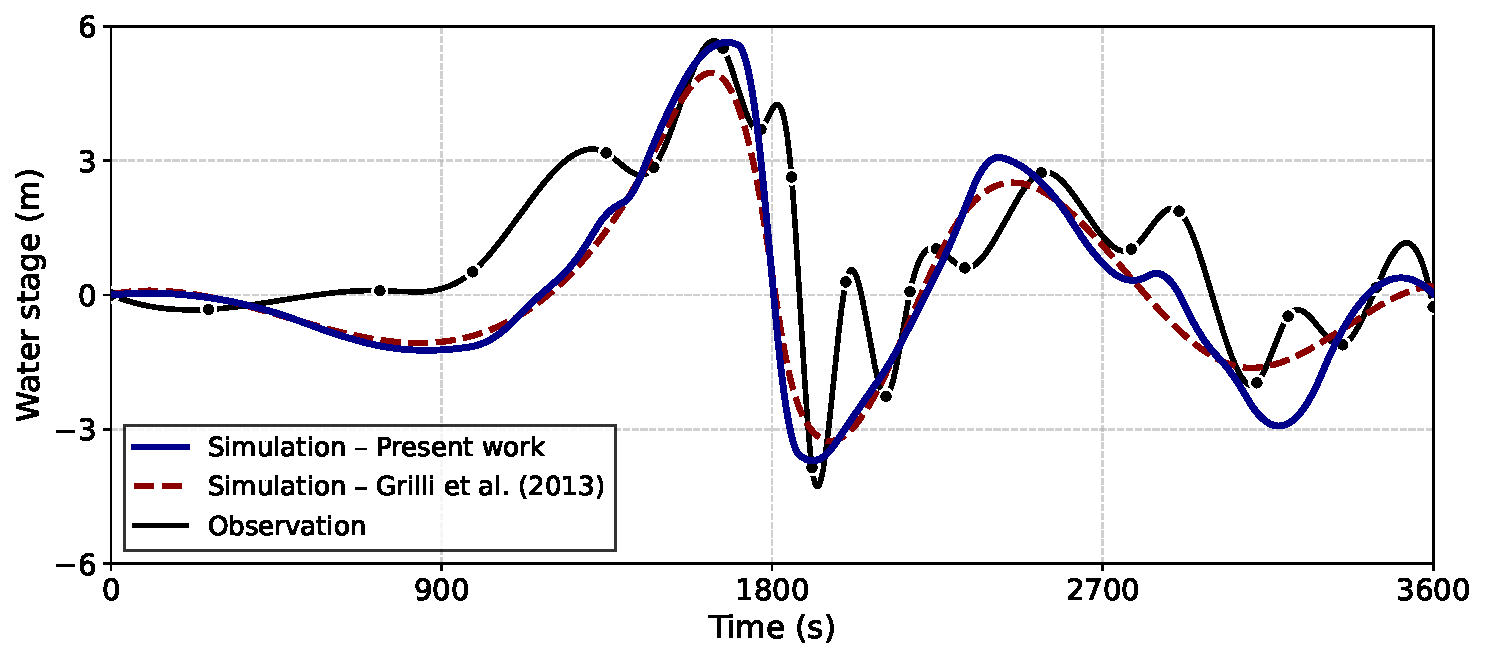
\includegraphics[width=0.9\textwidth]{Figuers/validation_gauge_g.pdf}
\caption{\scriptsize Comparison of simulated free-surface elevation time series at North Miyagi offshore GPS wave gauge (station 803, NOWPHAS network) with recorded measurements during the 2011 Tohoku tsunami.}
\label{fig:tohoku_validation}
\end{figure}


The dTSUNAMI results exhibit very good agreement with both the observed data and the reference simulation, accurately capturing the arrival time, amplitude of the leading crest, and the subsequent wave train. This close match clearly demonstrates the validity and high accuracy of the solver for real-world large-scale tsunami propagation simulations.







\subsection*{Adjoint-Based Sensitivity Computation}
\label{sec:adjoint_sensitivity}

To quantify the sensitivity of the final water depth \( h_N \) to variations in bed topography \( b \), we employ the adjoint method. This approach efficiently computes gradients without requiring finite-difference perturbations, making it well-suited for high-dimensional tsunami simulations.

\subsubsection*{Adjoint System Formulation}

The forward SWE system evolves as:
\begin{equation}
\mathbf{U}_{n+1} = \mathbf{U}_n + \frac{\Delta t_n}{2} \left( \mathbf{K}_1^n + \mathbf{K}_2^n \right),
\end{equation}
where
\begin{equation}
\mathbf{K}_1^n = \mathbf{F}(\mathbf{U}_n, \mathbf{b}), \quad
\mathbf{K}_2^n = \mathbf{F}(\widetilde{\mathbf{U}}_n, \mathbf{b}),
\end{equation}
and the final objective function is:
\begin{equation}
J = \mathbf{h}_N = \mathbf{P} \mathbf{U}_N,
\end{equation}
where \( \mathbf{P} \) extracts water depth \( h \) from \( \mathbf{U} \).

The Lagrangian function incorporates the constraints imposed by the forward dynamics:
\begin{align}
\mathcal{L} = J + \sum_{n=0}^{N-1} \bigg[
\boldsymbol{\lambda}_{1,n}^T \left( \mathbf{K}_1^n - \mathbf{F}(\mathbf{U}_n, \mathbf{b}) \right)
+ \boldsymbol{\lambda}_{2,n}^T \left( \widetilde{\mathbf{U}}_n - \mathbf{U}_n - \Delta t_n \mathbf{K}_1^n \right)  \notag \\
+ \boldsymbol{\lambda}_{3,n}^T \left( \mathbf{K}_2^n - \mathbf{F}(\widetilde{\mathbf{U}}_n, \mathbf{b}) \right)
+ \boldsymbol{\lambda}_{4,n}^T \left( \mathbf{U}_{n+1} - \mathbf{U}_n - \frac{\Delta t_n}{2} (\mathbf{K}_1^n + \mathbf{K}_2^n) \right) \bigg].
\end{align}

\subsubsection*{Backward Recursive Computation of Adjoint Variables}

The adjoint system is solved by backward recursion, starting from the final time step.

\textbf{Initialization at Final Time Step:}
\begin{equation}
\boldsymbol{\lambda}_{4,N-1} = -\mathbf{P}^T.
\end{equation}

\textbf{Recursive Computation for \( n = N-1, N-2, \dots, 0 \):}
\begin{enumerate}
    \item Compute adjoint correction for \( \mathbf{K}_2^n \):
    \begin{equation}
    \boldsymbol{\lambda}_{3,n} = \frac{\Delta t_n}{2} \boldsymbol{\lambda}_{4,n}.
    \end{equation}

    \item Compute adjoint variable for the intermediate state \( \widetilde{\mathbf{U}}_n \):
    \begin{equation}
    \boldsymbol{\lambda}_{2,n} = \boldsymbol{\lambda}_{3,n}^T \frac{\partial \mathbf{F}}{\partial \mathbf{U}} \Big|_{\widetilde{\mathbf{U}}_n}.
    \end{equation}

    \item Compute adjoint correction for \( \mathbf{K}_1^n \):
    \begin{equation}
    \boldsymbol{\lambda}_{1,n} = \Delta t_n \boldsymbol{\lambda}_{2,n} + \frac{\Delta t_n}{2} \boldsymbol{\lambda}_{4,n}.
    \end{equation}

    \item Update adjoint state for the next iteration:
    \begin{equation}
    \boldsymbol{\lambda}_{4,n-1} = \boldsymbol{\lambda}_{1,n} \frac{\partial \mathbf{F}}{\partial \mathbf{U}} \Big|_{\mathbf{U}_n} + \boldsymbol{\lambda}_{2,n} + \boldsymbol{\lambda}_{4,n}.
    \end{equation}
\end{enumerate}
The recursive computation of \(\boldsymbol{\lambda}\) proceeds from the final time step \(N\) back to the initial time step \(0\). The pseudocode for efficient implementation of the recursion is presented in Algorithm~\ref{alg:adjoint}.


\begin{algorithm}[H]
\caption{Recursive Computation of \(\boldsymbol{\lambda}\)}
\label{alg:adjoint}
\begin{algorithmic}[1]
    \State \textbf{Input:} 
    \begin{itemize}
        \item Time steps \(\Delta t_n\)
        \item Jacobians \(\frac{\partial \mathbf{F}}{\partial \mathbf{b}}\big|_{\mathbf{U}_n}\), \(\frac{\partial \mathbf{F}}{\partial \mathbf{b}}\big|_{\widetilde{\mathbf{U}}_n}\)
        \item Output matrix \(\mathbf{P}\)
    \end{itemize}
    \State \textbf{Initialize:} 
    \[
    \boldsymbol{\lambda}_{4,N-1} \gets -\mathbf{P}^T
    \]
    \For{\(n = N-1, N-2, \dots, 0\)}
        \State \textbf{Step 1: Compute \(\boldsymbol{\lambda}_{3,n}\)}
        \[
        \boldsymbol{\lambda}_{3,n} \gets \frac{\Delta t_n}{2} \boldsymbol{\lambda}_{4,n}
        \]

        \State \textbf{Step 2: Compute \(\boldsymbol{\lambda}_{2,n}\)}
        \[
        \boldsymbol{\lambda}_{2,n} \gets \boldsymbol{\lambda}_{3,n}^T \frac{\partial \mathbf{F}}{\partial \mathbf{U}} \big|_{\widetilde{\mathbf{U}}_n}
        \]

        \State \textbf{Step 3: Compute \(\boldsymbol{\lambda}_{1,n}\)}
        \[
        \boldsymbol{\lambda}_{1,n} \gets \Delta t_n \boldsymbol{\lambda}_{2,n} + \frac{\Delta t_n}{2} \boldsymbol{\lambda}_{4,n}
        \]

        \State \textbf{Step 4: Update \(\boldsymbol{\lambda}_{4,n-1}\)}
        \[
        \boldsymbol{\lambda}_{4,n-1} \gets \boldsymbol{\lambda}_{1,n} \frac{\partial \mathbf{F}}{\partial \mathbf{U}} \big|_{\mathbf{U}_n} + \boldsymbol{\lambda}_{2,n} + \boldsymbol{\lambda}_{4,n}
        \]

        \State \textbf{Step 5: Store Intermediate Values:}
        \begin{itemize}
            \item Save \(\boldsymbol{\lambda}_{1,n}\) for sensitivity computation
            \item Save \(\boldsymbol{\lambda}_{3,n}\) for sensitivity computation
        \end{itemize}
    \EndFor
\end{algorithmic}
\end{algorithm}

The final sensitivity of the water depth at \( t = T \) with respect to bed topography is obtained as:

\begin{equation}
\frac{\partial J}{\partial b} = \sum_{n=0}^{N-1} \left[
-\boldsymbol{\lambda}_{1,n}^T \frac{\partial \mathbf{F}}{\partial b} \Big|_{\mathbf{U}_n}
- \boldsymbol{\lambda}_{3,n}^T \frac{\partial \mathbf{F}}{\partial b} \Big|_{\widetilde{\mathbf{U}}_n}
\right].
\end{equation}

Since \( J = \mathbf{h}_N = \mathbf{P} \mathbf{U}_N \), we obtain:

\begin{equation}
\frac{\partial h_N}{\partial b} = \sum_{n=0}^{N-1} \left[
-\boldsymbol{\lambda}_{1,n}^T \frac{\partial \mathbf{F}}{\partial b} \Big|_{\mathbf{U}_n}
- \boldsymbol{\lambda}_{3,n}^T \frac{\partial \mathbf{F}}{\partial b} \Big|_{\widetilde{\mathbf{U}}_n}
\right].
\end{equation}

This Jacobian \( \frac{\partial h_N}{\partial b} \in \mathbb{R}^{M \times M} \) quantifies how changes in bed topography influence final water depth, crucial for tsunami inversion and forecasting.


\subsubsection*{Derivation of $\frac{\partial \mathbf{F}}{\partial \mathbf{U}}$ for FVM}
To compute the adjoint sensitivity, we derive the local Jacobian \( \frac{\partial \mathbf{F}}{\partial \mathbf{U}} \) for the finite volume discretization. Differentiating the numerical flux at a face shared between cells \( i \) and \( j \):

\begin{equation}
\frac{\partial \mathbf{F}_f}{\partial \mathbf{U}_i} =
\begin{pmatrix}
\mathbf{u} \cdot \mathbf{n} & n_x & n_y \\
u (\mathbf{u} \cdot \mathbf{n}) + g h n_x & 2 u n_x & u n_y \\
v (\mathbf{u} \cdot \mathbf{n}) + g h n_y & v n_x & 2 v n_y
\end{pmatrix}.
\end{equation}

For source terms including bed slope and friction:
\begin{equation}
\frac{\partial \mathbf{S}_i}{\partial \mathbf{U}_i} =
\begin{pmatrix}
0 & 0 & 0 \\
- g \frac{\partial b}{\partial x} - c_f u & -c_f |\mathbf{u}| & 0 \\
- g \frac{\partial b}{\partial y} - c_f v & 0 & -c_f |\mathbf{u}|
\end{pmatrix},
\end{equation}
where \( c_f = g n^2 / h^{4/3} \) is the friction coefficient.

\paragraph{Jacobian Assembly}
The full local Jacobian is assembled as:
\begin{equation}
\frac{\partial \mathbf{F}_i}{\partial \mathbf{U}_i} = -\frac{1}{A_i} \sum_{f \in \text{faces}(i)} l_f \frac{\partial \mathbf{F}_f}{\partial \mathbf{U}_i} + \frac{\partial \mathbf{S}_i}{\partial \mathbf{U}_i}.
\end{equation}
For neighboring cell interactions:
\begin{equation}
\frac{\partial \mathbf{F}_i}{\partial \mathbf{U}_j} = \frac{1}{A_i} l_f \frac{\partial \mathbf{F}_f}{\partial \mathbf{U}_j}, \quad j \in \text{neighbors}(i).
\end{equation}

This formulation ensures consistency with the adjoint framework, capturing local sensitivities required for gradient-based inversion and optimization.




\subsubsection*{Derivation of $\frac{\partial \mathbf{F}}{\partial b}$ for FVM}
To compute the local sensitivity of the shallow water system to bed topography \( b \), we differentiate the right-hand side function \( \mathbf{F} \).

\paragraph{Flux Contributions}
The governing equations include:
\begin{align}
\frac{\partial \mathbf{F}_1}{\partial b} &= 0, \\[5pt]
\frac{\partial \mathbf{F}_2}{\partial b} &= -gh \frac{\partial b}{\partial x}, \\[5pt]
\frac{\partial \mathbf{F}_3}{\partial b} &= -gh \frac{\partial b}{\partial y}.
\end{align}
Only the momentum equations contain explicit \( b \)-dependence via the bed slope terms.

For a domain with \( M \) cells, the Jacobian matrix is:
\begin{equation}
\frac{\partial \mathbf{F}}{\partial b} =
\begin{pmatrix}
\mathbf{0}_{M \times M} \\[5pt]
- g \text{diag}(h) \cdot \text{diag}(S_x) \\[5pt]
- g \text{diag}(h) \cdot \text{diag}(S_y)
\end{pmatrix} \in \mathbb{R}^{3M \times M}.
\end{equation}

In this formulation, the first \( M \) rows correspond to continuity equations with no explicit \( b \)-dependence. The middle and last \( M \) rows represent the effects of bed slope on x- and y-momentum equations, respectively. The diagonal form ensures each grid cell's sensitivity is localized, aligning with the adjoint system.



\subsection*{Neural Operator Learning for the Shallow Water Equations}

We employ neural operator learning to model tsunami dynamics governed by the shallow water equations with Manning friction, applied to the 2011 Tohoku event setup. Variability across samples arises from earthquake-induced seafloor deformation, represented through the Okada dislocation framework. Okada fault parameters are sampled within the ranges reported in \citep{grilli2013numerical}, and random earthquake epicenters are assigned as illustrated in Supplementary Fig.~\ref{fig:nse_sampling_strategies}.  

To generate training data, we used the dTSUNAMI finite volume solver on an unstructured triangular mesh consisting of 308,001 cells and 154,598 nodes. Each simulation is run for 3600 seconds, storing 51 uniformly spaced snapshots. These high-resolution solutions and their Jacobians are subsequently coarsened to a 100×100 uniform grid for neural operator training.

Within the SC-NO framework, the input function consists of the first $t_u = 5$ time steps of the water stage field $h(\mathbf{x}, t)$ together with the seafloor deformation $\Delta z_b(\mathbf{x})$ computed from the Okada model. The neural operator $\mathcal{G}_\theta$ is then trained to predict the remaining $t_G = 46$ time steps, guided by the Jacobian of the final water stage with respect to the bed topography, computed via the adjoint method (Supplementary Section~\ref{sec:adjoint_sensitivity}). Formally, the operator learning problem is defined as:
\begin{equation}
\mathcal{G}_\theta : \left( \mathcal{X} \times [0, t_u], \, \Delta z_b(\mathbf{x}) \right) \;\to\; h(\mathbf{x}, t, \Delta z_b), 
\quad \text{for } (\mathbf{x}, t) \in \mathcal{X} \times [t_u, T].
\end{equation}

To evaluate both interpolation and extrapolation performance, we consider two testing scenarios: (i) an \textit{in-training} case, where earthquake epicenters fall within the range covered by the training set, and (ii) an \textit{out-of-training} case, where epicenters lie outside this region (Supplementary Fig.~\ref{fig:nse_sampling_strategies}). This setup enables us to assess not only the accuracy of SC-NO within the training distribution but also its ability to generalize tsunami propagation to previously unseen earthquake configurations, serving as an out-of-distribution (OOD) evaluation.  


This approach integrates spatial-temporal input information with earthquake source parameters, enabling SC-NO to learn a solution operator that generalizes tsunami propagation and inundation across both in-training and out-of-distribution epicenter scenarios.  


\begin{figure}[!ht]
    \centering
    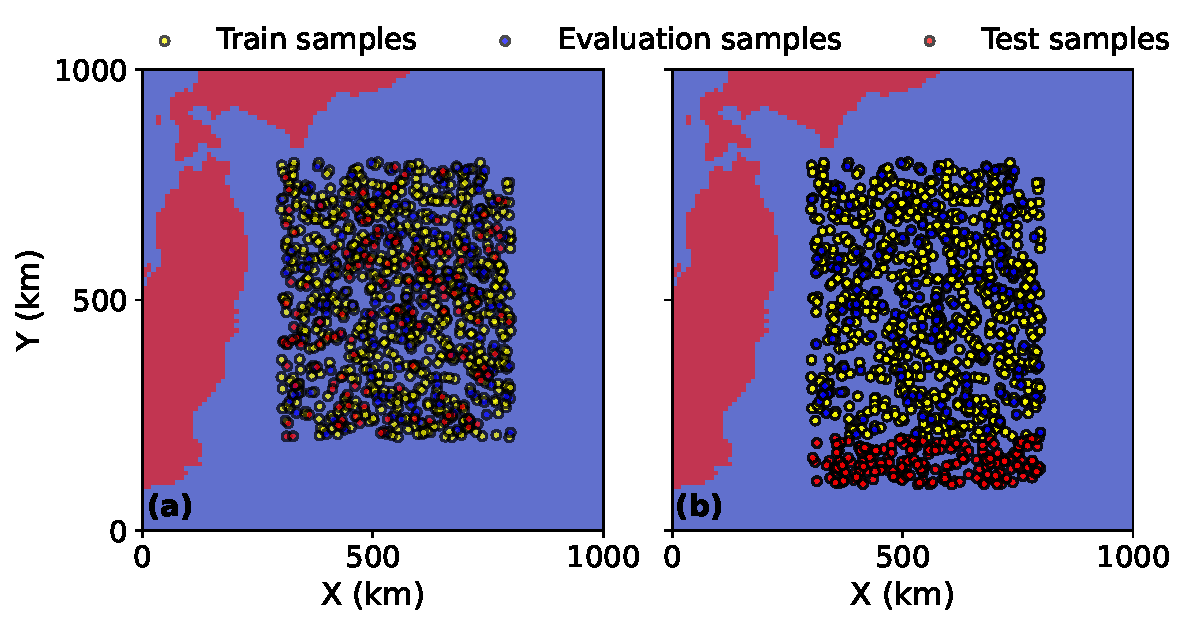
\includegraphics[width=0.8\textwidth]{Figuers/sampling_strategy.pdf}

    \caption{\scriptsize\textbf{Sampling strategy for PDE3 (tsunami scenario).} 
    (a) Training and evaluation samples are generated from random earthquake epicenters distributed across the central region of the domain. 
    (b) Out-of-distribution (OOD) test samples are generated by shifting epicenters into a geographically distinct southern band, ensuring that all test events occur in a region not represented in the training or evaluation sets.}     
        
        \label{fig:nse_sampling_strategies}
\end{figure}




\subsection*{Mapping Between Fine Solver Mesh and Coarse Neural Operator Grid}
\label{sec:coarse_fine_mapping}

For the shallow-water tsunami case (PDE3), neural operator training and inference are conducted on a fixed $100\times100$ uniform grid, while the governing dynamics are solved on a substantially finer unstructured mesh using the dTSUNAMI finite volume solver. This resolution disparity requires two complementary mappings: a \emph{coarsening} operator that restricts high-resolution solutions to the learning grid, and an \emph{upscaling} operator that reconstructs physically consistent fine-scale fields from coarse neural-operator predictions.

\paragraph{Coarsening of fine-scale solutions.}
Let $d(\mathbf{x}, t)$ denote the fine-scale water depth field produced by the solver on the continuous domain $\mathcal{X}$. We introduce a uniform partition $\{\Omega_{ij}\}$ of $\mathcal{X}$ corresponding to the $100\times100$ neural operator grid. Coarsening is performed via a cell-averaging operator,
\begin{equation}
\bar{d}_{ij}(t)
=
\frac{1}{|\Omega_{ij}|}
\int_{\Omega_{ij}} d(\mathbf{x}, t)\, d\mathbf{x},
\end{equation}
yielding a coarse depth field $\bar{d}_{ij}(t)$ that preserves the mean water depth within each cell. In practice, this corresponds to averaging solver values associated with fine mesh elements whose centroids lie within $\Omega_{ij}$. This projection provides a physically consistent low-resolution representation suitable for neural operator learning while retaining the dominant large-scale dynamics.




\paragraph{Physically based upscaling from coarse to fine resolution.}
The inverse mapping from coarse mean depth to fine-scale depth is not uniquely defined: many fine configurations yield the same coarse average. To obtain a physically meaningful reconstruction, the upscaling is defined as a \emph{cell-wise hydrostatic fill} over the known fine bathymetry.

Let $\{\Omega_{ij}\}$ denote the $100\times 100$ coarse partition of the horizontal domain, and let $\{(\mathbf{x}_p,z_{b,p})\}_{p=1}^{N}$ be the fine solver nodes (or vertices), where $\mathbf{x}_p\in\mathbb{R}^2$ and $z_{b,p}=z_b(\mathbf{x}_p)$ is the bed elevation. Each fine node is assigned to exactly one coarse cell via
\begin{equation}
c(p)= (i,j)\quad \text{s.t.}\quad \mathbf{x}_p\in\Omega_{ij}, 
\qquad 
\mathcal{P}_{ij}=\{p:\,c(p)=(i,j)\},\quad N_{ij}=|\mathcal{P}_{ij}|.
\end{equation}
The neural operator predicts the coarse mean depth $\bar d_{ij}(t)$ on each cell. The reconstructed fine depth is defined pointwise by
\begin{equation}
d_p(t) \;=\; \big(H_{ij}(t)-z_{b,p}\big)_+,
\qquad p\in\mathcal{P}_{ij},
\qquad (a)_+ := \max(a,0),
\label{eq:bathtub_pointwise}
\end{equation}
where $H_{ij}(t)$ is a \emph{cell-wise water level} (stage) chosen to satisfy the coarse mean-depth constraint in \emph{discrete} form:
\begin{equation}
\frac{1}{N_{ij}}\sum_{p\in\mathcal{P}_{ij}} \big(H_{ij}(t)-z_{b,p}\big)_+ \;=\; \bar d_{ij}(t).
\label{eq:bathtub_mean_constraint}
\end{equation}
Equation~\eqref{eq:bathtub_mean_constraint} defines $H_{ij}(t)$ implicitly. The left-hand side is a continuous, non-decreasing function of $H_{ij}(t)$, hence the solution exists and is unique whenever $\bar d_{ij}(t)$ is attainable over the local bathymetric distribution $\{z_{b,p}\}_{p\in\mathcal{P}_{ij}}$. In practice, $H_{ij}(t)$ is obtained by bisection with brackets
\begin{equation}
H_{ij}^{\mathrm{low}} = \min_{p\in\mathcal{P}_{ij}} z_{b,p},
\qquad
H_{ij}^{\mathrm{high}} = \max_{p\in\mathcal{P}_{ij}} z_{b,p} + \bar d_{ij}(t) + \varepsilon,
\end{equation}
and the cell is treated as dry whenever $\bar d_{ij}(t)\le d_{\min}$, in which case $d_p(t)=0$ for all $p\in\mathcal{P}_{ij}$.

Finally, to ensure that the reconstruction preserves the \emph{total} water volume implied by the coarse prediction at each time $t$, an optional per-time-step global rescaling is applied. Let $A_{ij}=|\Omega_{ij}|$ be the coarse cell area and approximate each node in $\Omega_{ij}$ by an equal area weight $A_{ij}/N_{ij}$. Then the target and reconstructed volumes are
\begin{equation}
V_{\mathrm{target}}(t)=\sum_{i,j} \bar d_{ij}(t)\,A_{ij},
\qquad
V_{\mathrm{rec}}(t)=\sum_{i,j}\sum_{p\in\mathcal{P}_{ij}} d_p(t)\,\frac{A_{ij}}{N_{ij}},
\end{equation}
and we set a scalar factor $\alpha(t)=V_{\mathrm{target}}(t)/V_{\mathrm{rec}}(t)$ (when $V_{\mathrm{rec}}(t)>0$) and replace $d_p(t)\leftarrow \alpha(t)\,d_p(t)$.
This upscaling is therefore non-negative, bathymetry-aware, and exactly consistent with the coarse mean-depth constraints by construction, while avoiding the unphysical shoreline behavior that can arise from purely geometric interpolation in shallow regions.



\begin{figure}[!ht]
    \centering
    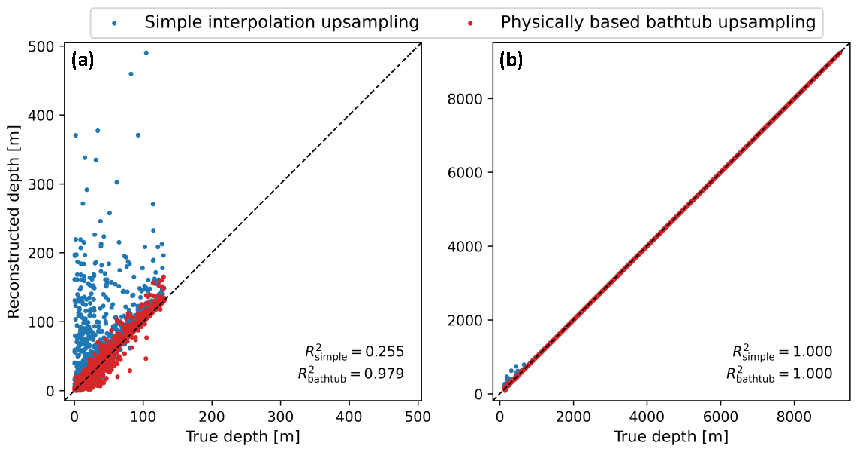
\includegraphics[width=0.9\textwidth]{Figuers/upsampling_error.pdf}
    \caption{\scriptsize\textbf{Comparison of depth upscaling methods.}
    (a) Shallow-water regime (0--5th percentile of true depth).
    (b) Moderate-to-deep regime (5--100th percentile of true depth).}
    \label{fig:upsampling_comparison}
\end{figure}




A common alternative is to upsample coarse predictions using standard interpolation methods (e.g., nearest-neighbor or bilinear interpolation of depth or stage). Such approaches ignore bathymetric variability and do not enforce physical constraints, often leading to spurious inundation over dry land and degraded accuracy in shallow regions.

Figure~\ref{fig:upsampling_comparison} illustrates a controlled comparison between a standard interpolation-based reconstruction and the proposed physically based upscaling procedure. Starting from a high-resolution reference solution obtained from the tsunami solver, the water depth field is first \emph{coarsened} to the $100\times100$ uniform grid used by the neural operator. This coarse representation is then independently upscaled back to the original fine resolution using (i) a purely geometric interpolation scheme and (ii) the proposed bathtub-based reconstruction. The resulting reconstructed fields are compared against the original high-resolution solution.

In shallow-water regions near the shoreline (0–5th percentile of true depth), interpolation-based reconstruction fails to recover physically meaningful depths and exhibits poor agreement with the reference solution (Figure~\ref{fig:upsampling_comparison}a). This failure arises because interpolation does not account for local bathymetric structure and cannot enforce essential physical constraints such as non-negativity of depth or shoreline emergence. In contrast, the bathtub-based reconstruction explicitly incorporates the underlying bed elevation and enforces consistency with the coarse mean depth, yielding accurate recovery of shallow-water states.

In moderate-to-deep regions, both reconstruction approaches perform comparably well, indicating that simple interpolation is sufficient only away from the shoreline (Figure~\ref{fig:upsampling_comparison}b). These results demonstrate that physically informed upscaling is a necessary complement to coarse neural-operator predictions when reconstructing near-shore and inundation-relevant tsunami dynamics, while purely geometric interpolation is inadequate in depth regimes most critical for hazard assessment.
Taken together, this comparison establishes the upscaling procedure as a reliable and physically consistent complement to the neural-operator framework. While SC-NO is trained and evaluated entirely on coarse-resolution fields, the proposed reconstruction enables faithful recovery of fine-scale depth distributions required for solver-level validation, visualization, and downstream hazard analysis. Importantly, this post-processing step operates independently of the learned operator and does not modify its predictions; instead, it provides a principled bridge between coarse neural-operator outputs and high-resolution physical fields, ensuring consistency with bathymetry and shallow-water physics.





\subsection*{Three-Stage Inversion Framework for Tsunami Source Reconstruction}
\label{sec:inversion_framework}

Rapid and reliable estimation of tsunami sources is vital for the effectiveness of real-time early-warning systems. When a major undersea earthquake occurs, the resulting seafloor deformation initiates tsunami waves that can traverse ocean basins and reach coastal regions within minutes, demanding immediate and accurate source characterization.  
To meet this need, we introduce a \textbf{data-driven, gradient-based inversion framework} that integrates \textbf{Neural Operators} with \textbf{Okada surrogate networks} to reconstruct the earthquake-induced seafloor deformation and infer the corresponding fault parameters directly from \textbf{early-stage tsunami gauge observations}.  
These early observations, typically spanning the first 30 minutes after the event onset, contain limited yet highly informative signals that guide the inversion toward physically consistent, interpretable, and computationally efficient source reconstructions suitable for real-time forecasting.
The framework combines the differentiability and efficiency of neural operators with the interpretability of Okada fault parameterization, enabling near--real-time source reconstruction with both accuracy and physical coherence. The inversion proceeds in three sequential stages, progressively transitioning from field-level reconstruction to interpretable parameter refinement (Figure~\ref{fig:inversion_stages}).




\begin{figure}[htbp]
    \centering
    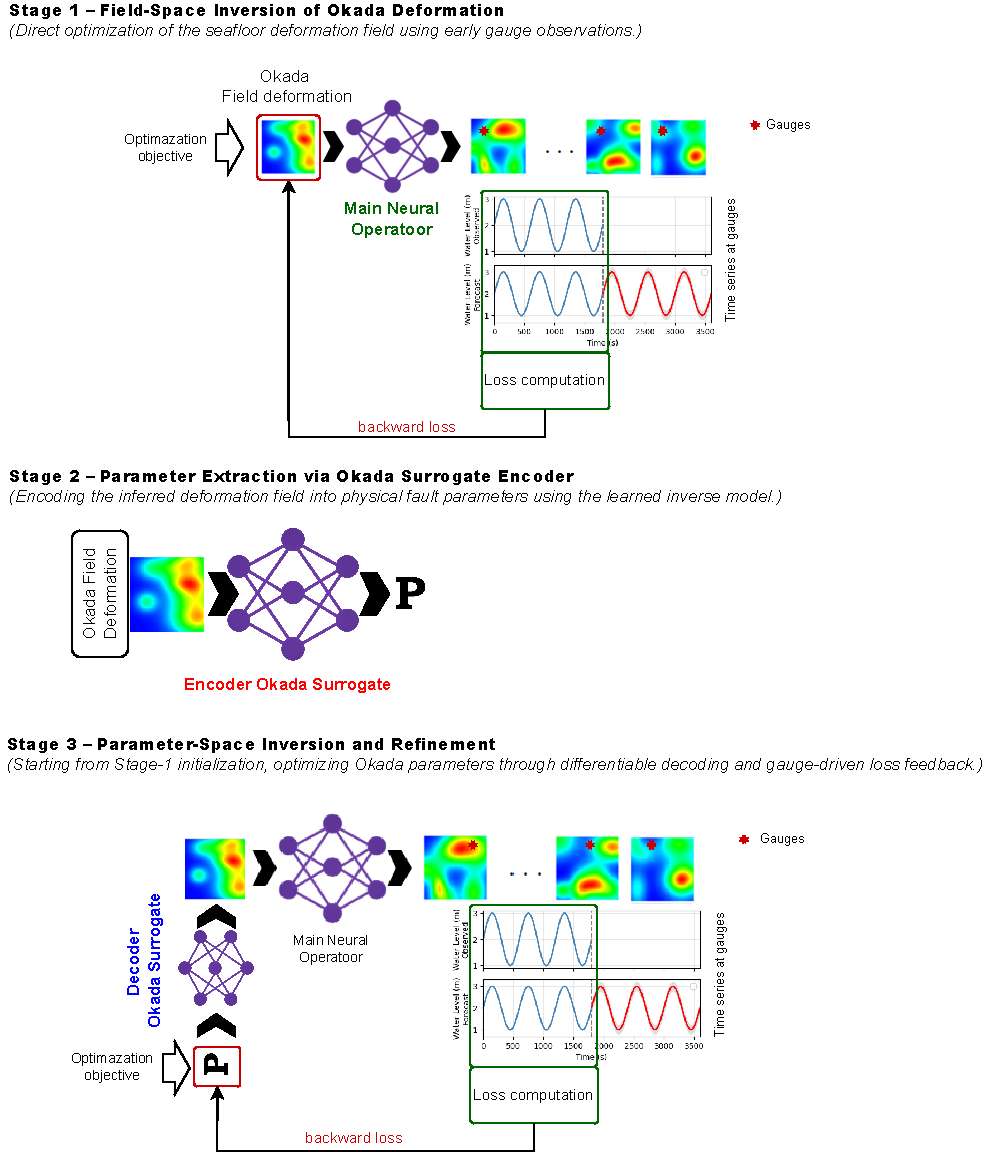
\includegraphics[width=0.98\textwidth, trim={0 0 0 0}, clip]{Figuers/inversion_tsunami.pdf}
    \caption{\scriptsize\textbf{Three-stage tsunami inversion workflow.}  
    The framework integrates neural operator surrogates and Okada-based encoder–decoder networks for rapid and interpretable tsunami source reconstruction.  
    \textbf{Stage~1:} Field-space inversion optimizes the Okada deformation field using early tsunami gauge observations via neural operator surrogates (FNO or SC-FNO).  
    \textbf{Stage~2:} The inferred deformation is passed through a U-FNO--based Okada Surrogate Encoder that maps the 2D field to a nine-dimensional fault parameter vector $\mathbf{P}$.  
    \textbf{Stage~3:} A U-FNO Decoder reconstructs the deformation field from $\mathbf{P}$, enabling parameter-space refinement through differentiable feedback and gauge-driven loss propagation.
    }
    
    \label{fig:inversion_stages}
\end{figure}



\begin{figure}[htbp]
    \centering
    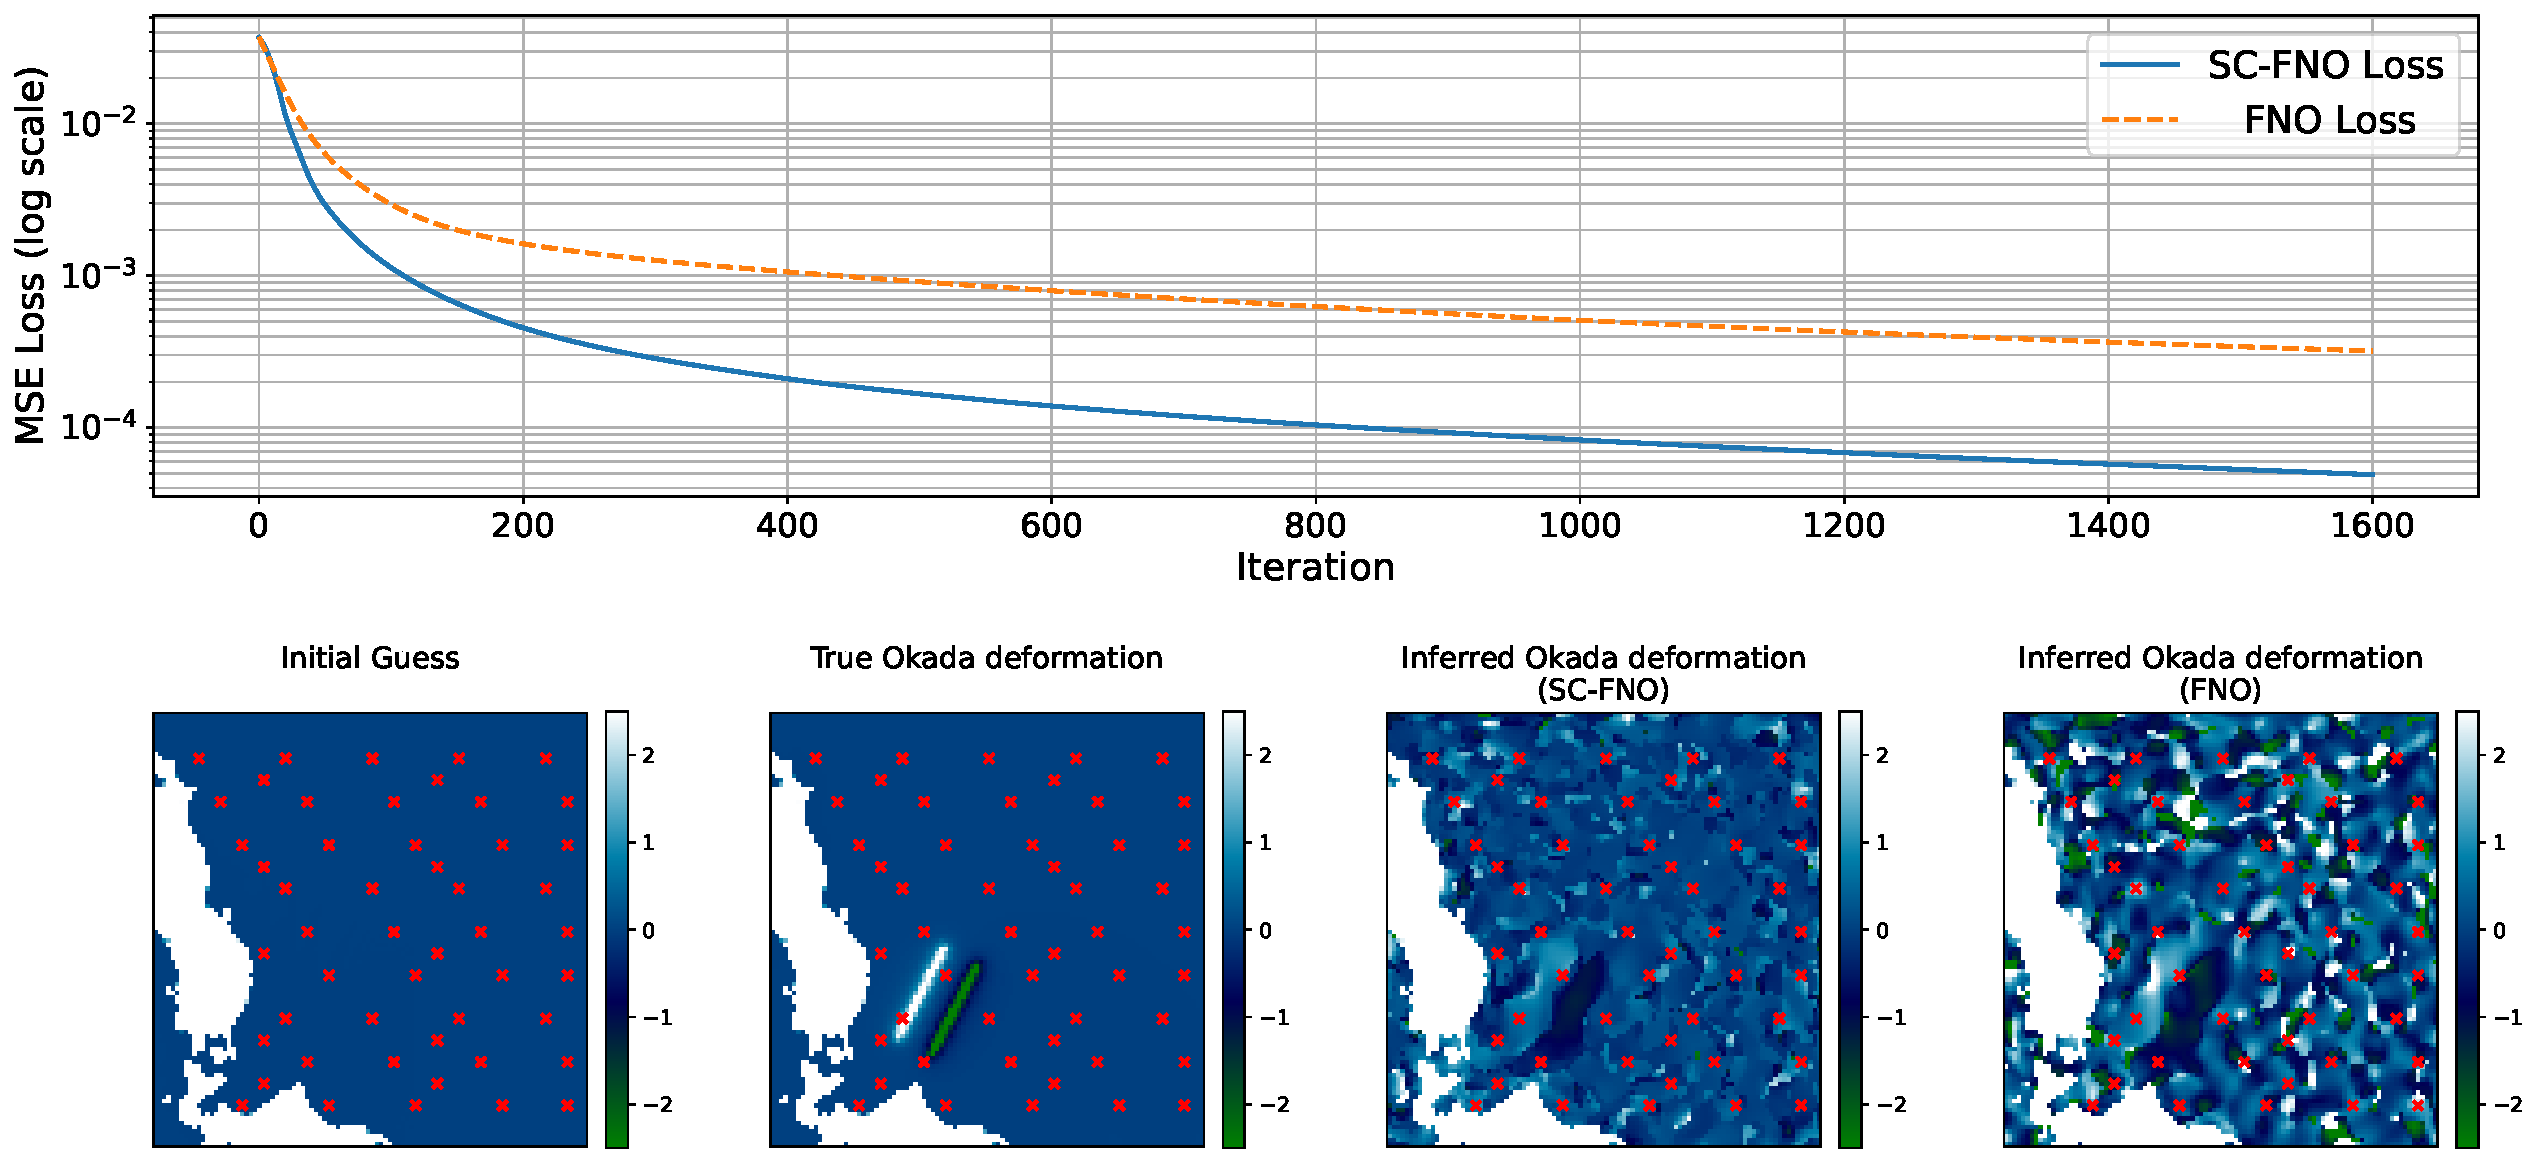
\includegraphics[width=\textwidth, trim={0 0 0 0}, clip]{Figuers/PDE3_inversion_stage_1.pdf}
    \caption{\scriptsize\textbf{Field-space inversion of Okada deformation (Stage~1).}  
    Evolution of the mean squared error (MSE) loss during inversion using SC-FNO and FNO (top), and comparison of deformation fields (bottom).  
    Red dots indicate the locations of tsunami gauges.}
        \label{fig:stage1_field_inversion}
\end{figure}




\paragraph{Stage 1 --- Field-Space Inversion of Okada Deformation}
\textit{(Direct gradient-based optimization of the seafloor deformation field using early gauge observations.)}

In the first stage, inversion is performed directly in the \textbf{field domain} to reconstruct the Okada deformation field---the vertical displacement of the seafloor responsible for tsunami initiation.  
Starting from an initial guess, the deformation field is iteratively updated through gradient descent to minimize the mean squared error between simulated and observed water-stage time series at selected gauge locations during the early event window ($T_u = 30$ minutes).  

Forward simulations are produced by a pretrained Neural Operator---either the baseline FNO or the Sensitivity-Constrained FNO ---which acts as a differentiable surrogate for the shallow water equations.  
This stage yields an initial deformation estimate that reproduces the observed signals but may contain \textbf{low-frequency artifacts} or \textbf{nonphysical features}, since the optimization acts directly on spatial pixels without explicit parameter constraints. At the end of Stage~1, both models converge toward deformation fields that reproduce the early tsunami gauge observations with reasonable accuracy (Figure~\ref{fig:stage1_field_inversion}). Although residual discrepancies remain in both reconstructions, the \textbf{SC-FNO} demonstrates faster convergence, smoother gradients, and more accurate localization of the primary rupture zone compared to the baseline \textbf{FNO}. The SC-FNO–inferred field better captures the overall geometry, polarity, and region of occurrence of the true Okada deformation, while the FNO result remains affected by high-frequency noise and scattered artifacts.  




\paragraph{Stage 2 --- Parameter Extraction via Okada Surrogate Encoder}
\textit{(Encoding the inferred deformation field into compact Okada fault parameters through a learned inverse mapping.)}

To restore physical interpretability, the deformation field recovered in Stage~1, denoted as $\mathbf{F} \in \mathbb{R}^{H \times W}$, is passed through a pretrained \textbf{Okada Surrogate Encoder} $E_{\theta}$.  
This network performs the nonlinear mapping  
\[
E_{\theta} : \mathbf{F} \; \rightarrow \; \mathbf{P} \in \mathbb{R}^{9},
\]
where $\mathbf{P}$ represents the compact vector of Okada fault parameters, including the fault epicenter coordinates ($x$, $y$), depth, length, width, strike, dip, rake, and slip magnitude.



% Although purely data-driven and not physics-informed, this pair effectively approximates the analytical mapping. The encoding step compresses the field inversion result into a physically constrained latent representation, ensuring that subsequent optimization evolves along a \textbf{realistic fault manifold} while suppressing spatial artifacts from Stage~1.



\begin{figure}[htbp]
    \centering
    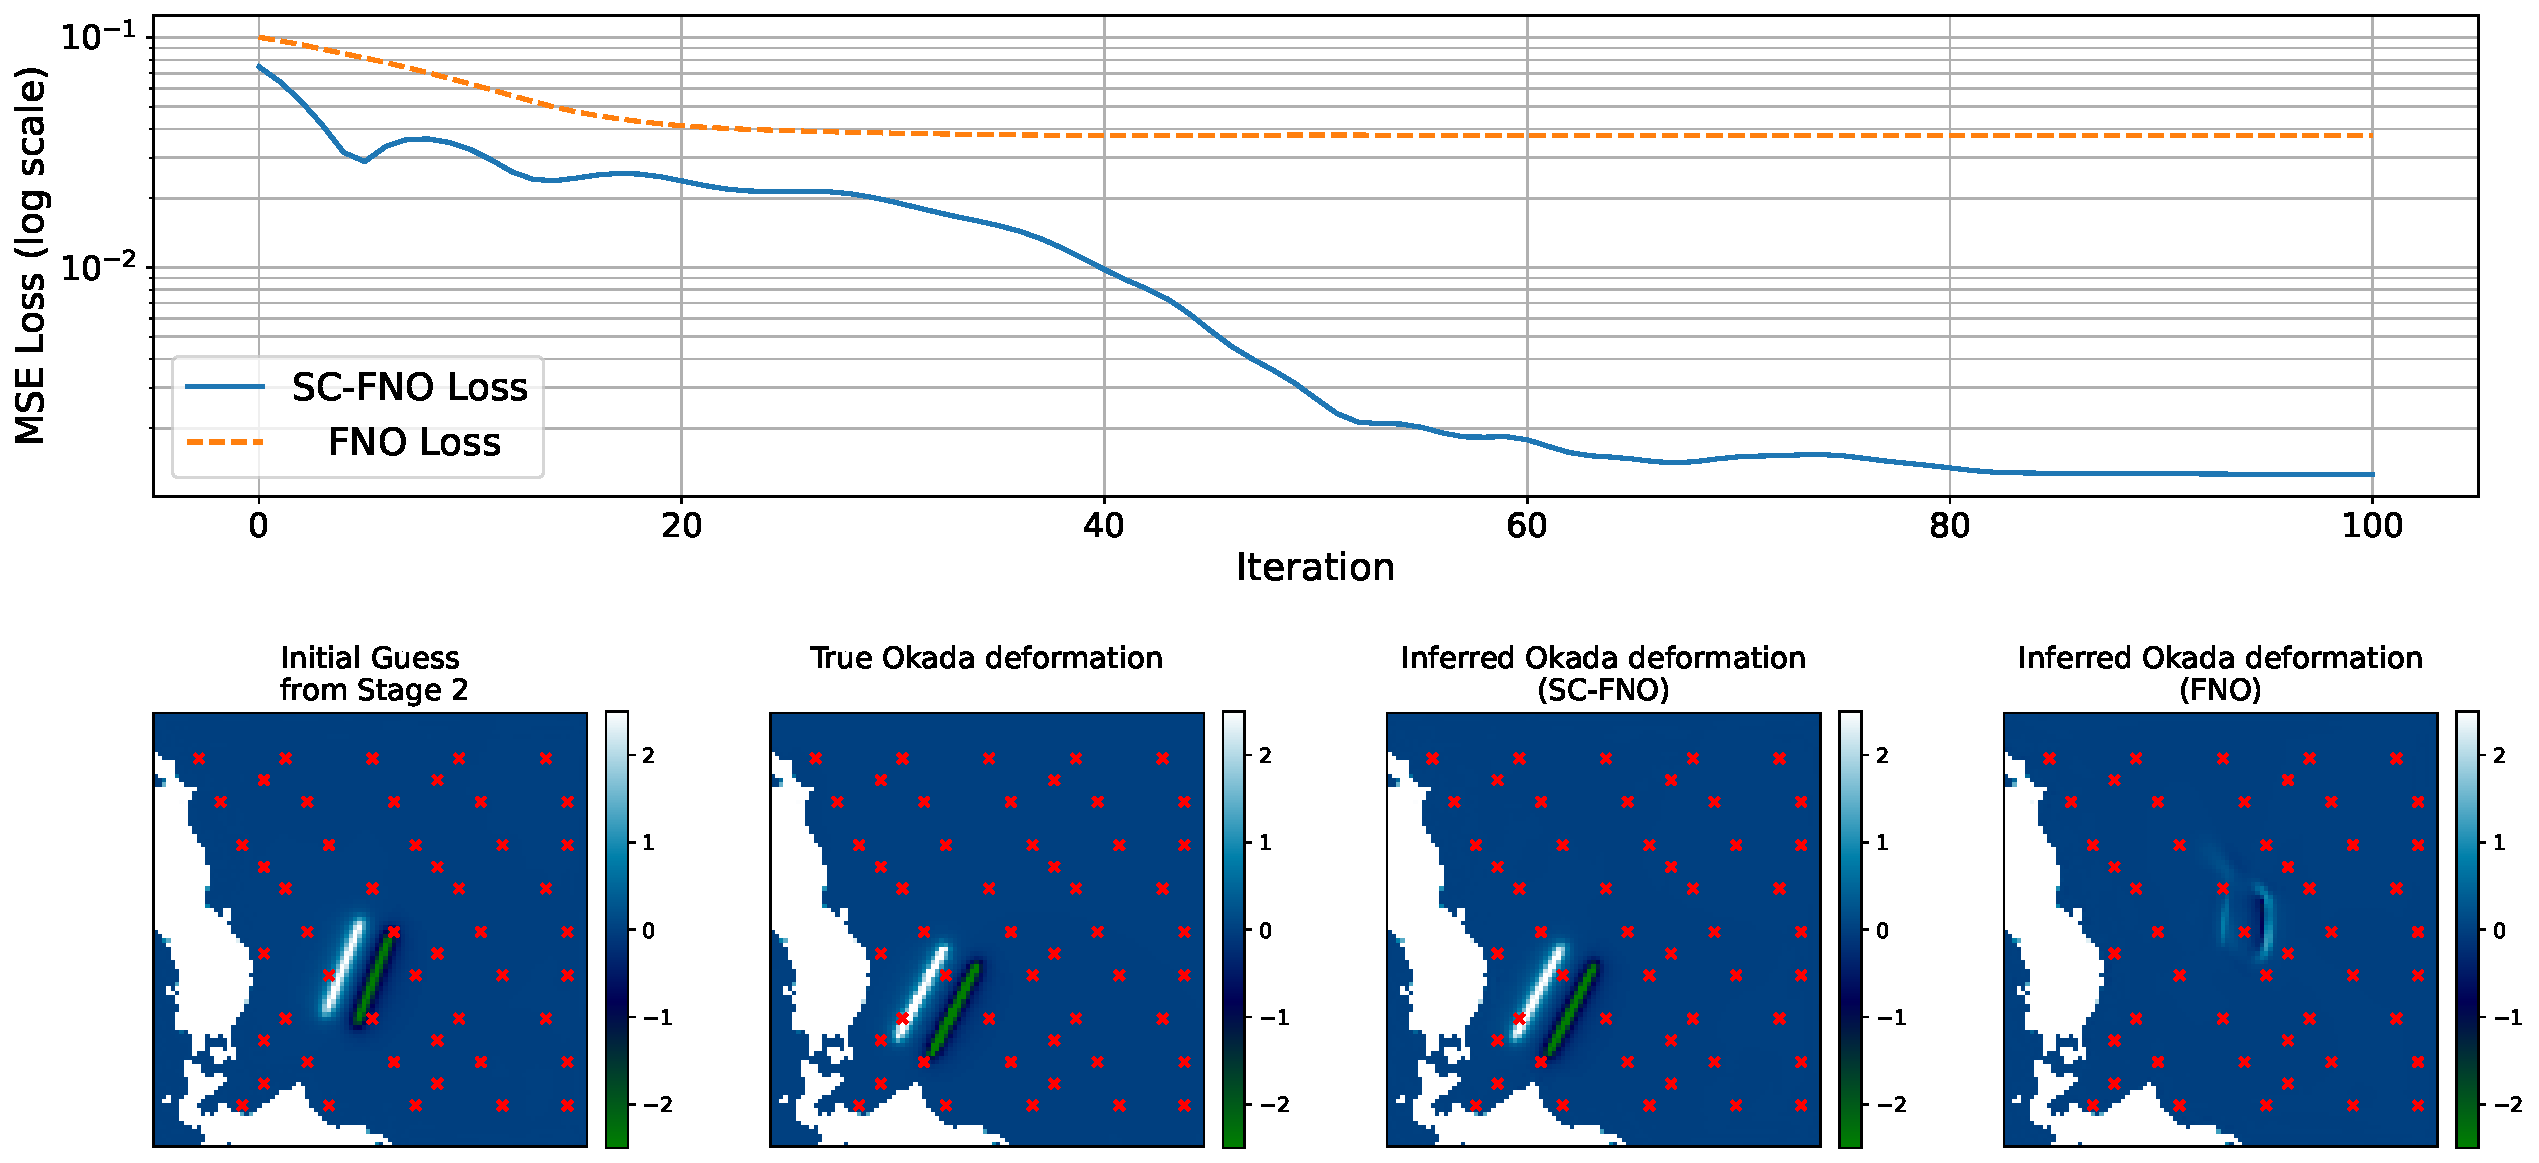
\includegraphics[width=0.98\textwidth, trim={0 0 0 0}, clip]{Figuers/PDE3_inversion_stage_2.pdf}
    \caption{\scriptsize\textbf{Parameter-space inversion and refinement (Stage~3).}  
    Convergence of the mean squared error (MSE) loss during parameter-space optimization (top) and comparison of deformation fields (bottom).  
    The optimization is initialized using parameters inferred from Stage~2 and refined through the differentiable Decoder Okada Surrogate.  
    The sensitivity-constrained neural operator (SC-FNO) achieves faster convergence and higher reconstruction fidelity compared to the baseline FNO, closely reproducing the true Okada deformation.  
    Red dots indicate tsunami gauge locations.}
    \label{fig:stage3_param_inversion}
\end{figure}



\paragraph{Stage 3 --- Parameter-Space Inversion and Refinement via Decoder Okada Surrogate}
\textit{(Gradient-based optimization of Okada parameters using differentiable decoding and gauge-driven feedback.)}

In the final stage, inversion operates in the \textbf{parameter domain}. The vector $\mathbf{P}$ obtained from Stage~2 serves as the initial guess for a new optimization loop. A pretrained \textbf{Decoder Okada Surrogate} maps $\mathbf{P}$ back into its corresponding seafloor deformation field, providing a differentiable link between the parameters and simulated tsunami signals.  

At each iteration, the decoded deformation field is propagated through the main neural operator (FNO or SC-FNO) to generate gauge predictions. The resulting loss between predicted and observed signals is backpropagated through the full pipeline---decoder and forward model included---to update all nine Okada parameters simultaneously via gradient descent.  
This stage refines the parameter estimates within a physically meaningful subspace, producing deformation fields that are dynamically consistent with observed data.


At the end of Stage~3, the inversion converges toward a stable and physically consistent solution (Figure~\ref{fig:stage3_param_inversion}).
While the baseline \textbf{FNO} fails to achieve meaningful refinement, the \textbf{SC-FNO} continues to reduce the residual mismatch between predicted and observed gauge signals, converging toward the true Okada deformation. The resulting field accurately recovers both the location and polarity of the rupture with minimal spatial artifacts, confirming that sensitivity-constrained learning enables effective parameter-space optimization and physically reliable reconstruction.



With the final Okada deformation field inferred from Stage~3, the complete tsunami evolution can now be simulated through the trained neural operator model. By propagating the recovered deformation through the \textbf{FNO} and \textbf{SC-FNO} forward models, we reconstruct the full spatiotemporal dynamics of the event from the initial seafloor motion to the final coastal impact.
Representative tsunami gauge time series are shown in Figure~\ref{fig:gauge_timeseries}, demonstrating that while both models reproduce the overall waveform trends, the \textbf{SC-FNO} achieves closer agreement with observed amplitudes and phases, maintaining stability and reducing residual errors throughout the simulation.


\begin{figure}[htbp]
\centering
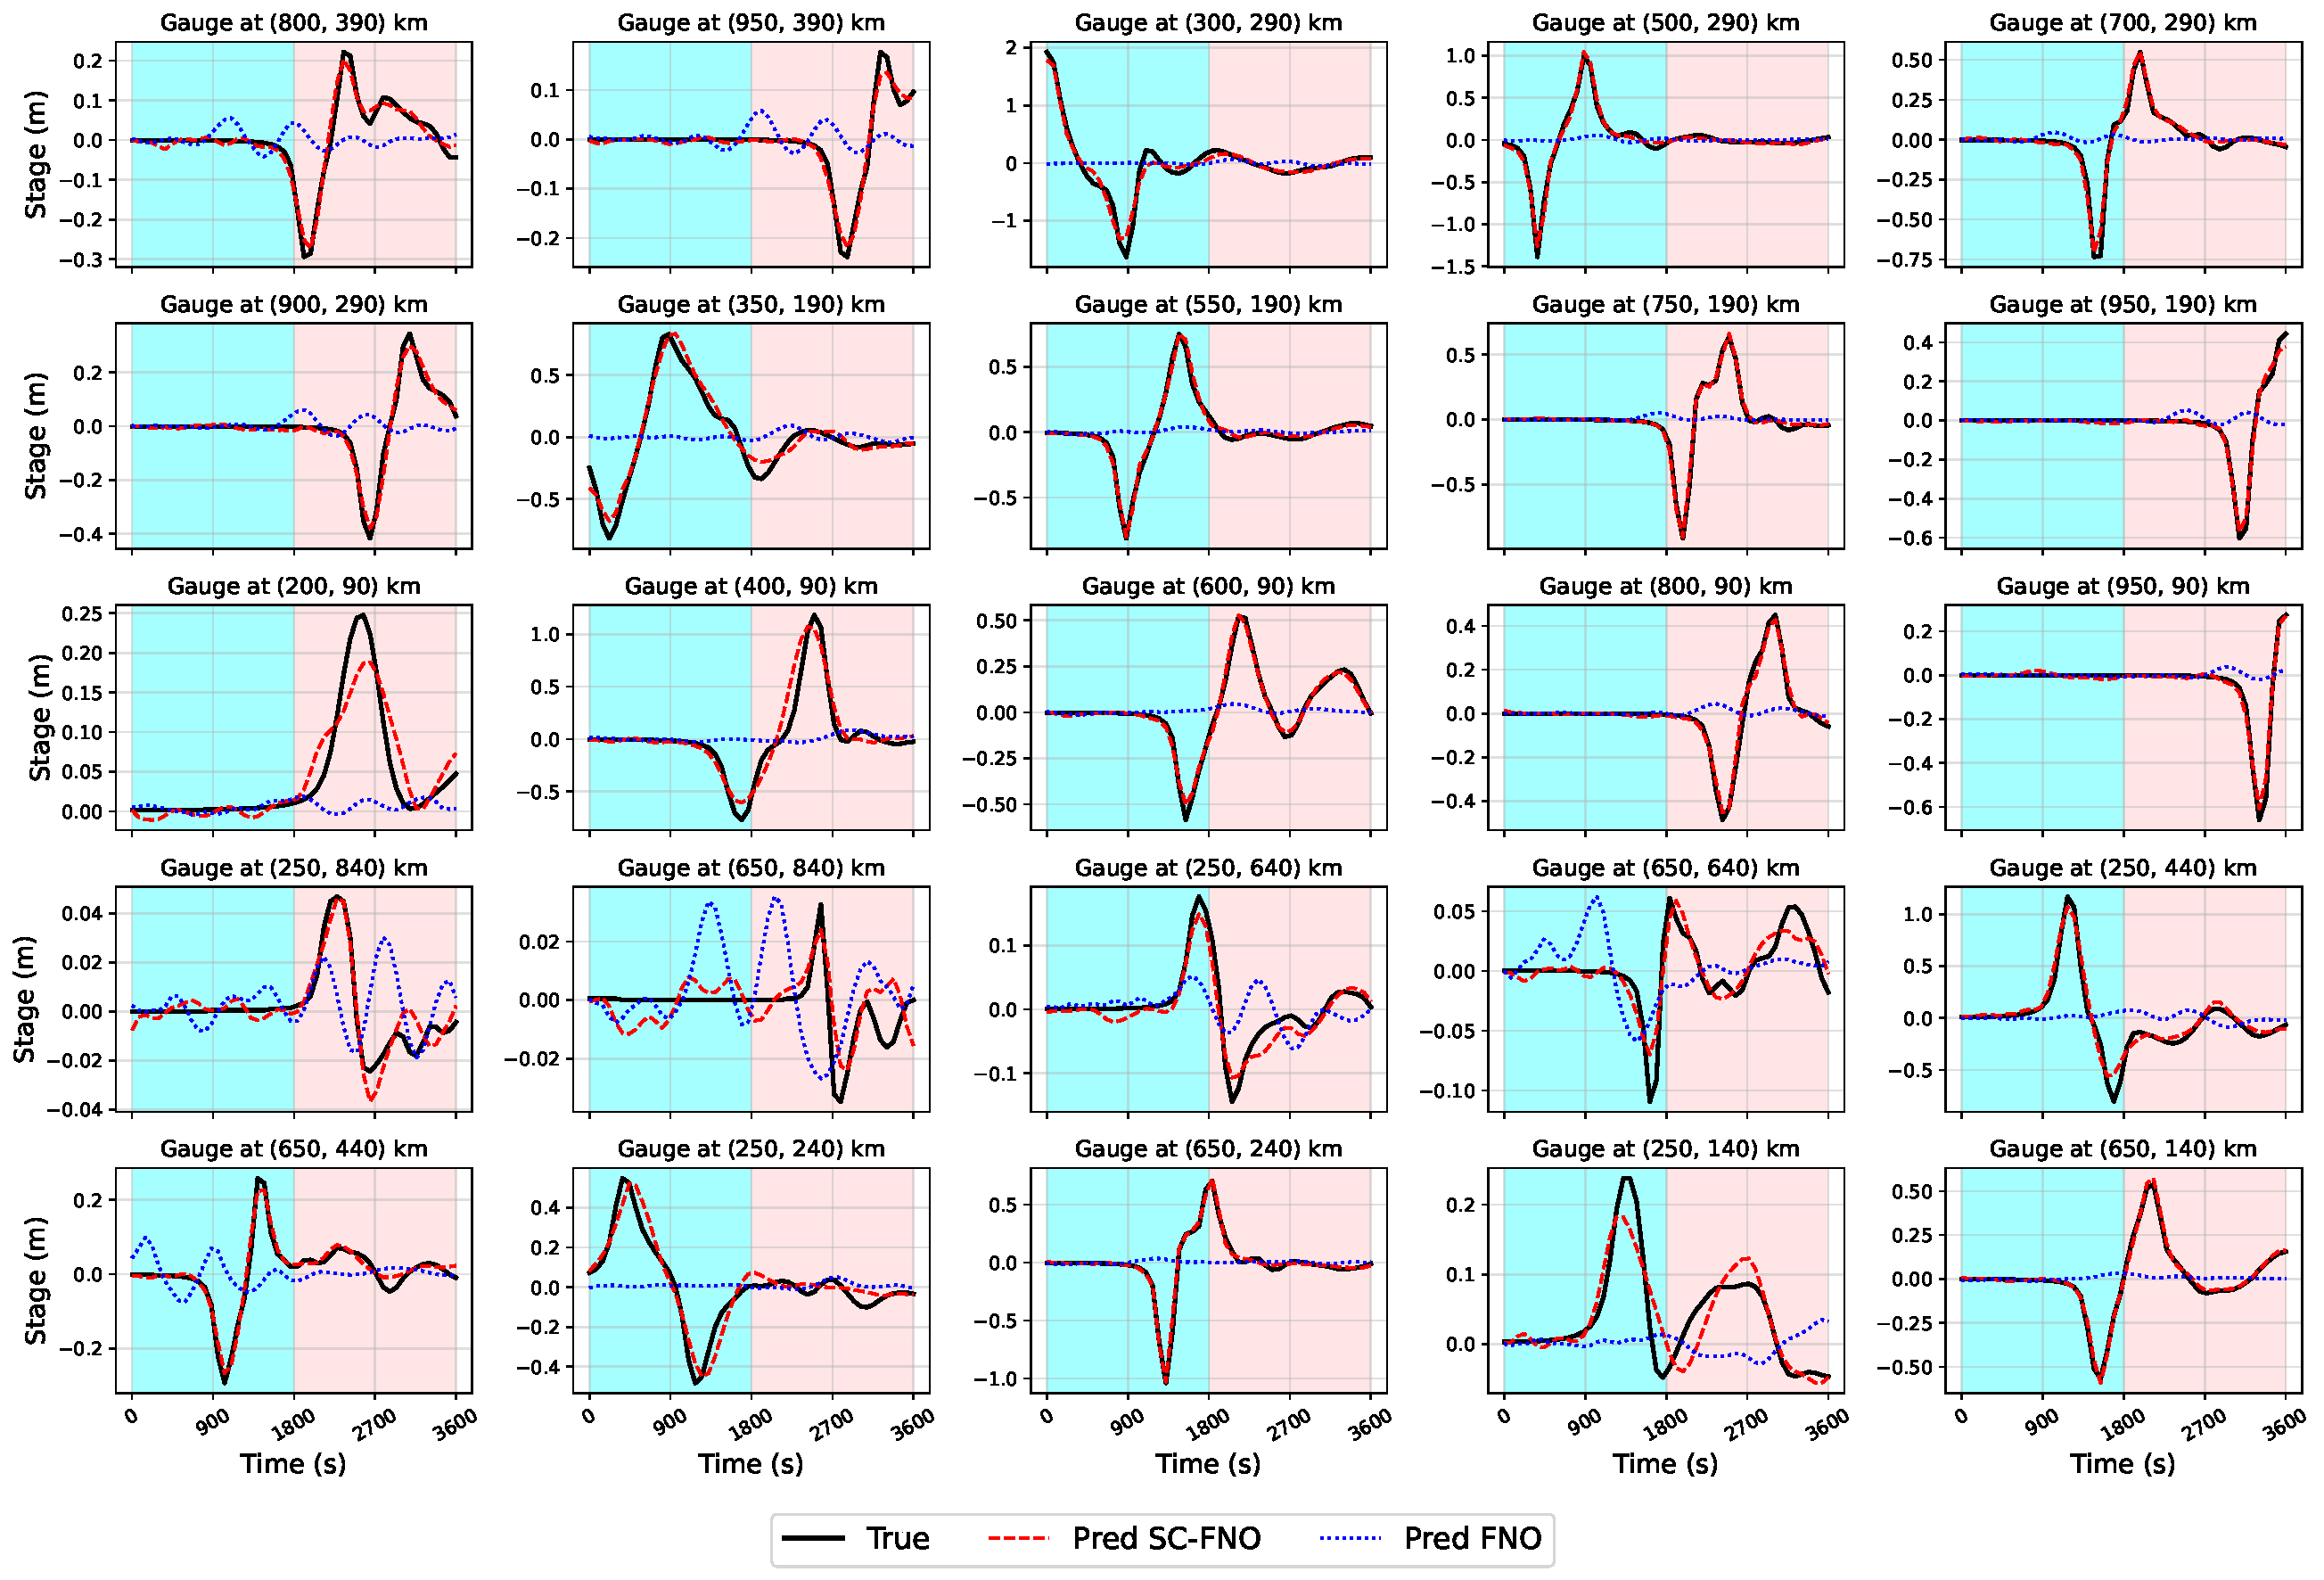
\includegraphics[width=0.98\textwidth, trim={0 0 0 0}, clip]{Figuers/PDE3_sensor_history.pdf}
\caption{\scriptsize\textbf{Reconstructed tsunami gauge time series using the inferred Okada deformation.} Comparison between observed (black), SC-FNO predictions (red dashed), and FNO predictions (blue dotted) at multiple gauge locations. The aqua-shaded regions denote the early portion of the event ($T_u = 30$,min) used as input for inversion, while the light-red regions represent the unseen time window predicted by the models.
}
\label{fig:gauge_timeseries}
\end{figure}




\subsection*{Additional results for PDE3}

% Table for performances of models for forward prediction of PDE3 
\begin{table}[htbp]
\centering
\caption{\scriptsize\textbf{Comparison of Error Metrics Across Models Trained with Different Sample Sizes (in-training) PDE3}}
\label{tab:pde3_forward_nostd}
\scriptsize
\setlength{\tabcolsep}{3pt}
\begin{tabular}{lcccccccc}
\hline
\textbf{Model} & \multicolumn{2}{c}{\textbf{1200 Samples}} & \multicolumn{2}{c}{\textbf{1000 Samples}} & \multicolumn{2}{c}{\textbf{700 Samples}} & \multicolumn{2}{c}{\textbf{200 Samples}} \\
 & \textbf{Rel. \(L^2\)} & \textbf{MAE} & \textbf{Rel. \(L^2\)} & \textbf{MAE} & \textbf{Rel. \(L^2\)} & \textbf{MAE} & \textbf{Rel. \(L^2\)} & \textbf{MAE} \\
\hline
FNO        & \(7.1 \times 10^{-2}\) & \(6.8 \times 10^{-2}\) & \(8.9 \times 10^{-2}\) & \(7.6 \times 10^{-2}\) & \(1.12 \times 10^{-1}\) & \(9.2 \times 10^{-2}\) & \(5.9 \times 10^{-1}\) & \(5.8 \times 10^{-1}\) \\
WNO        & \(7.6 \times 10^{-2}\) & \(7.3 \times 10^{-2}\) & \(9.5 \times 10^{-2}\) & \(8.1 \times 10^{-2}\) & \(1.18 \times 10^{-1}\) & \(9.9 \times 10^{-2}\) & \(6.3 \times 10^{-1}\) & \(6.2 \times 10^{-1}\) \\
DeepONet   & \(8.2 \times 10^{-2}\) & \(7.9 \times 10^{-2}\) & \(1.01 \times 10^{-1}\) & \(8.7 \times 10^{-2}\) & \(1.25 \times 10^{-1}\) & \(1.0 \times 10^{-1}\) & \(6.7 \times 10^{-1}\) & \(6.7 \times 10^{-1}\) \\
SC-FNO     & \(\mathbf{1.1 \times 10^{-2}}\) & \(\mathbf{2.2 \times 10^{-2}}\) & \(\mathbf{2.8 \times 10^{-2}}\) & \(\mathbf{5.6 \times 10^{-2}}\) & \(\mathbf{6.2 \times 10^{-2}}\) & \(\mathbf{1.0 \times 10^{-1}}\) & \(\mathbf{1.3 \times 10^{-1}}\) & \(\mathbf{2.3 \times 10^{-1}}\) \\
SC-WNO     & \(1.2 \times 10^{-2}\) & \(2.4 \times 10^{-2}\) & \(3.0 \times 10^{-2}\) & \(5.9 \times 10^{-2}\) & \(6.5 \times 10^{-2}\) & \(1.1 \times 10^{-1}\) & \(1.4 \times 10^{-1}\) & \(2.5 \times 10^{-1}\) \\
SC-DeepONet& \(1.5 \times 10^{-2}\) & \(2.8 \times 10^{-2}\) & \(3.6 \times 10^{-2}\) & \(7.0 \times 10^{-2}\) & \(7.1 \times 10^{-2}\) & \(1.2 \times 10^{-1}\) & \(1.6 \times 10^{-1}\) & \(2.9 \times 10^{-1}\) \\
\hline
\end{tabular}
\end{table}

% Table for performances of models for forward prediction of PDE3 (out-of-training / OOD)
\begin{table}[htbp]
\centering
\caption{\scriptsize\textbf{Comparison of Error Metrics Across Models Trained with Different Sample Sizes (out-of-training) PDE3}}
\label{tab:pde3_forward_ood}
\scriptsize
\setlength{\tabcolsep}{3pt}
\begin{tabular}{lcccccccc}
\hline
\textbf{Model} & \multicolumn{2}{c}{\textbf{1200 Samples}} & \multicolumn{2}{c}{\textbf{1000 Samples}} & \multicolumn{2}{c}{\textbf{700 Samples}} & \multicolumn{2}{c}{\textbf{200 Samples}} \\
 & \textbf{Rel. \(L^2\)} & \textbf{MAE} & \textbf{Rel. \(L^2\)} & \textbf{MAE} & \textbf{Rel. \(L^2\)} & \textbf{MAE} & \textbf{Rel. \(L^2\)} & \textbf{MAE} \\
\hline
FNO        & \(1.3 \times 10^{-1}\) & \(1.1 \times 10^{-1}\) & \(1.6 \times 10^{-1}\) & \(1.3 \times 10^{-1}\) & \(1.9 \times 10^{-1}\) & \(1.6 \times 10^{-1}\) & \(7.5 \times 10^{-1}\) & \(6.5 \times 10^{-1}\) \\
WNO        & \(1.4 \times 10^{-1}\) & \(1.2 \times 10^{-1}\) & \(1.8 \times 10^{-1}\) & \(1.4 \times 10^{-1}\) & \(2.1 \times 10^{-1}\) & \(1.7 \times 10^{-1}\) & \(8.0 \times 10^{-1}\) & \(6.9 \times 10^{-1}\) \\
DeepONet   & \(1.5 \times 10^{-1}\) & \(1.3 \times 10^{-1}\) & \(1.9 \times 10^{-1}\) & \(1.5 \times 10^{-1}\) & \(2.3 \times 10^{-1}\) & \(1.9 \times 10^{-1}\) & \(8.5 \times 10^{-1}\) & \(7.2 \times 10^{-1}\) \\
SC-FNO     & \(\mathbf{3.5 \times 10^{-2}}\) & \(\mathbf{6.0 \times 10^{-2}}\) & \(\mathbf{5.0 \times 10^{-2}}\) & \(\mathbf{8.0 \times 10^{-2}}\) & \(\mathbf{8.0 \times 10^{-2}}\) & \(\mathbf{1.0 \times 10^{-1}}\) & \(\mathbf{2.5 \times 10^{-1}}\) & \(\mathbf{3.0 \times 10^{-1}}\) \\
SC-WNO     & \(3.8 \times 10^{-2}\) & \(6.5 \times 10^{-2}\) & \(5.3 \times 10^{-2}\) & \(8.5 \times 10^{-2}\) & \(8.5 \times 10^{-2}\) & \(1.1 \times 10^{-1}\) & \(2.7 \times 10^{-1}\) & \(3.2 \times 10^{-1}\) \\
SC-DeepONet& \(4.2 \times 10^{-2}\) & \(7.0 \times 10^{-2}\) & \(5.7 \times 10^{-2}\) & \(9.0 \times 10^{-2}\) & \(9.5 \times 10^{-2}\) & \(1.2 \times 10^{-1}\) & \(3.0 \times 10^{-1}\) & \(3.5 \times 10^{-1}\) \\
\hline
\end{tabular}
\end{table}
